\chapter{Projeto e Implementação}\label{chap:projeto-implementacao}
Neste capítulo, entraremos em mais detalhes da parte de projeto e implementação do sistema, com base nos requisitos já levantados, passando pelas tecnologias envolvidas e pela arquitetura do sistema.

\section{Elaboração e Estrutura do Sistema}
Está seção explica, com mais detalhes, os casos de uso do sistema, as responsabilidades em comum entre cada um deles e como isso pode ser estruturado na arquitetura.

\subsection{Casos de Uso}
Com bases nos requisitos levantados anteriormente, foram construídos os casos de uso a seguir (para mais detalhes, ver o apêndice \ref{chap:use-case-appendix}):

\begin{itemize}
    \item Propor tema de trabalho: Alunos e Orientadores propõem temas em busca de orientadores ou alunos dispostos a realizarem.
    \item Login: Alunos, Orientadores, Co-orientadores e Coordenadores acessam sistema de maneira tradicional ou via Senha Única USP (para pertencentes à USP).
    \item Cadastrar disciplinas: Coordenadores cadastram a disciplina, os alunos participantes e as atividades.
    \item Editar disciplinas: Coordenadores editam disciplinas, cadastrando atividades, editando alunos etc.
    \item Cadastrar grupos de trabalhos: Coordenadores cadastram os grupos com os temas e os orientadores, com a confirmação da participação do orientador no grupo.
    \item Cadastrar professores: Coordenadores cadastram professores do departamento que podem orientar/co-orientar.
    \item Cadastrar pessoas externas: Coordenadores cadastram convidados do sistema que podem avaliar projetos nas bancas práticas e/ou co-orientar.
    \item Entregar atividade: Alunos submetem no Google Drive arquivos da atividade para a leitura do orientador, co-orientador e coordenadores.
    \item Listar entregas: Técnicos recebem os arquivos de impressão, com normalização do título, separados por grupo.
    \item Listar necessidades adicionais: Técnicos recebem necessidades adicionais revisadas pelos orientadores, separadas por grupo.
    \item Construir bancas práticas: Coordenadores selecionam os participantes da banca prática, já cadastrados no sistema, e os notifica com comentários sobre o evento.
    \item Construir bancas teóricas: Coordenadores escolhem participantes da banca teórica do grupo, selecionam o presidente da banca, realizam o agendamento do horário, validando inconsistências (participante já possui horário ocupado) e notificam os participantes por e-mail.
    \item Avaliar projetos práticos: Participantes da banca prática avaliam os projetos que estão envolvidos, limitando avaliações até o final do dia.
    \item Avaliar monografias teóricas: Participantes da banca teórica avaliam as monografias que estão envolvidas, gerando comentários e definindo o status do trabalho (aprovado, aprovado com correções, recuperação e reprovado), limitando avaliações até o final do dia.
    \item Calcular nota final dos projetos: Coordenadores determinam a fórmula para calcular as notas finais, com base nas entregas parciais durante as duas disciplinas e o sistema calcula as notas finais de todos os grupos participantes.
    \item Importar projetos aprovados: Sistema importa monografias revisadas, banners, press-releases, posters e links do site para a base de dados históricos de TCC.
    \item Cadastrar projetos avulsos: Coordenadores cadastram monografias revisadas, banners, press-releases, posters e links do site de trabalhos anteriores para a base de dados históricos de TCC.
    \item Buscar projetos anteriores: Usuários externos ao sistema procuram monografias anteriores, de acordo com o nome, ano, turma (semestral ou quadrimestral) e palavras-chave.
    \item Buscar temas propostos: Alunos e orientadores procuram temas propostos por outros alunos e orientadores, de acordo com o nome, palavras-chave e grupos de pesquisa do departamento, podendo se inscrever nas vagas para esses temas (se houverem).
\end{itemize}

\subsection{Diagramas de Casos de Uso}
Os casos de uso foram estruturados nos seguintes diagramas (elaborados com a ajuda da ferramenta PlantText \cite{planttext2018}, para ver como elas foram geradas, ver apêndice \ref{chap:use-case-appendix}):

\begin{figure}[H]
    \centering
    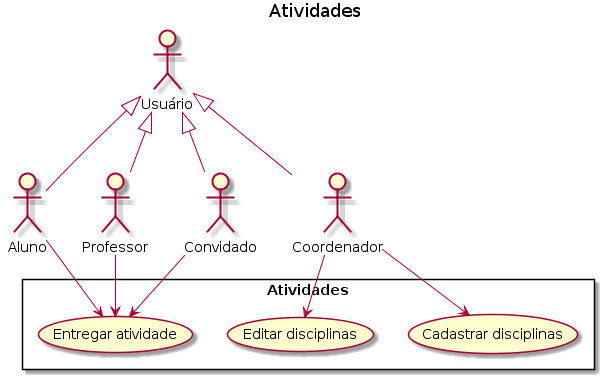
\includegraphics[scale=0.6]{atv.png}
    \caption{Diagrama de Casos de Uso para Atividades}
    \label{fig:use-case-atv}
\end{figure}

\begin{figure}[H]
    \centering
    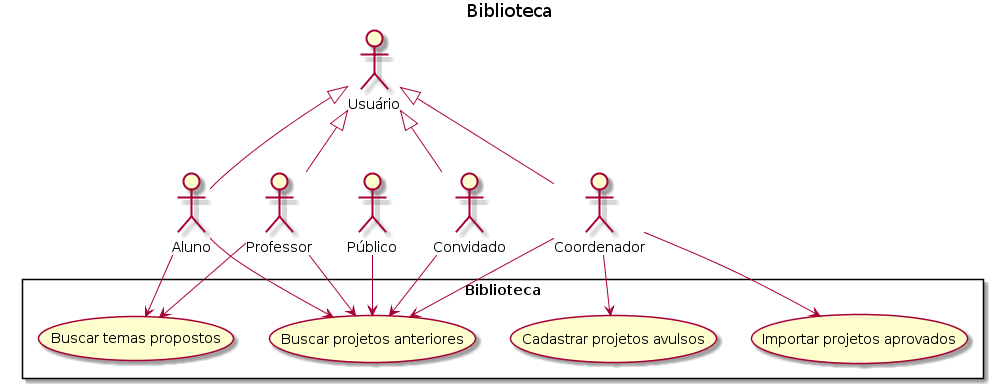
\includegraphics[scale=0.4]{bib.png}
    \caption{Diagrama de Casos de Uso para Base de Dados (Biblioteca Virtual)}
    \label{fig:use-case-atv}
\end{figure}

\begin{figure}[H]
    \centering
    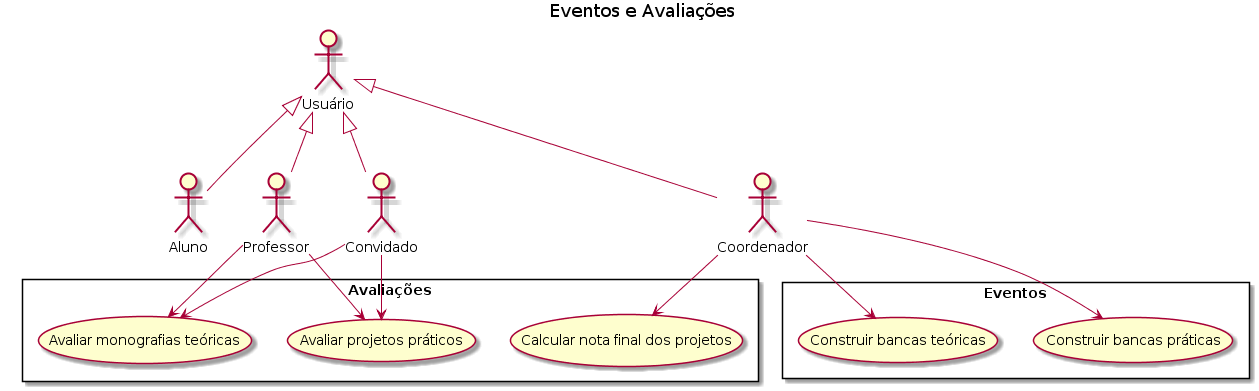
\includegraphics[scale=0.3]{ev-ava.png}
    \caption{Diagrama de Casos de Uso para Eventos e Avaliações}
    \label{fig:use-case-atv}
\end{figure}

\begin{figure}[H]
    \centering
    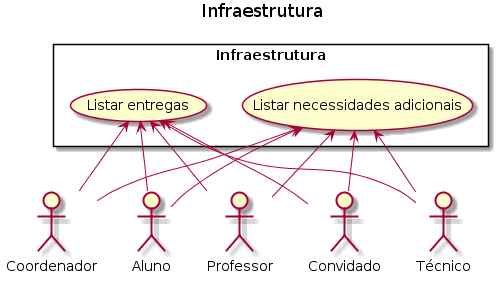
\includegraphics[scale=0.6]{infra.png}
    \caption{Diagrama de Casos de Uso para Infraestrutura}
    \label{fig:use-case-atv}
\end{figure}

\begin{figure}[H]
    \centering
    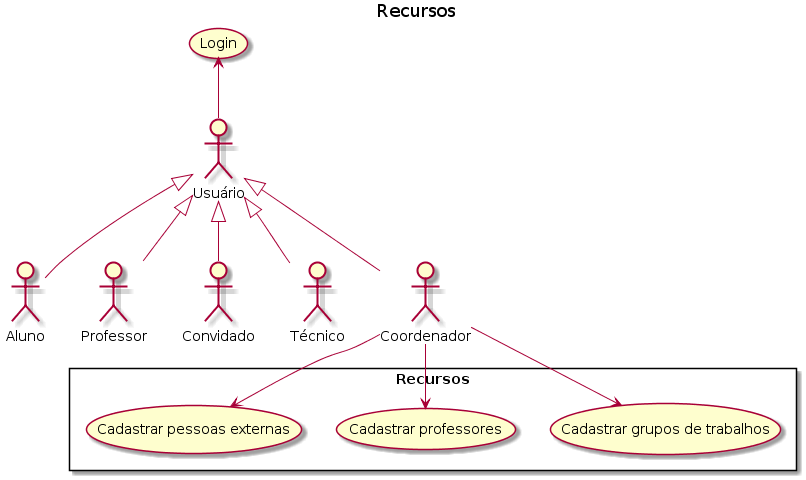
\includegraphics[scale=0.5]{recursos.png}
    \caption{Diagrama de Casos de Uso para Gerenciamento dos Recursos}
    \label{fig:use-case-atv}
\end{figure}

\section{Tecnologias Utilizadas}
Após determinar os requisitos do sistema e estabelecer os casos de uso, resta determinar as tecnologias a serem usadas, bem como a arquitetura do sistema.

Como parte dos requisitos, era necessário o uso de sistemas \textit{web} para os \textit{stakeholders} terem maior mobilidade e facilidade ao realizarem as interações com o sistema. Sendo assim, é valido passar por alguns conceitos tecnológicos do projeto.

\subsection{\textit{Frameworks web} e o Django}
É comum, em desenvolvimento de sistemas, usar soluções prontas como forma de simplificar o desenvolvimento de soluções. Essas soluções são conhecidas como arcabouços (ou \textit{frameworks})\cite{iansommerville2011}: "Um framework é uma estrutura genérica estendida para se criar uma aplicação ou subsistema mais específico.". Para este projeto, foi usado um \textit{framework}, em linguagem Python, chamado \textbf{Django}.

O Django é estruturado em aplicações (apps), onde cada aplicação corresponde a uma parte do sistema, geralmente independente e reciclável (ou seja, pode ser usada em aplicações Django diferentes). Cada aplicação segue o padrão \textit{Model-View-Controller}.

O padrão \textit{Model-View-Controller} - MVC é um padrão arquitetural para organizar os componentes da aplicação. Ele é dividido em três grandes grupos\cite{thedjangobook2018}:

\begin{itemize}
    \item Modelo (\textit{Model}): Uma representação (interface) para os dados da aplicação.
    \item Visualização (\textit{View}): Camada de apresentação dos dados da aplicação. No caso do Django, ele é chamado de \textit{Template}.
    \item Controlador (\textit{Controller}): Camada de controle que interliga o modelo com a apresentação dos dados, onde geralmente fica a lógica de negócio. No caso do Django, ele é conhecido como \textit{View}.
\end{itemize}

A vantagem do padrão está no fluxo de dados que existe entre os grupos, além de evitar códigos com funcionalidades diferentes em lugares errados, como, por exemplo, lógica de negócio na camada de apresentação.

\subsection{Arquitetura}
O Django foi usado na versão mais recente estável (2.1), que corrigiu algumas novidades da versão 2.0. É esta versão que foi usada pelo projeto em questão, dado que é estável e possui suporte de apoio da equipe até Dezembro de 2020\cite{djangodownload}. Ele usa, como padrão, o SQLite, o que atendeu bem durante o desenvolvimento. Já o Heroku tem como banco de dados padrão o PostgreSQL, o que exigiu o chaveamento entre os bancos no ambiente local de desenvolvimento e os ambientes de validação hospedados no serviço. Por isso, o projeto possui configurado dois pacotes de gerenciamento de banco de dados, um para SQLite (nativo do Django), outro para PostgreSQL (o Psycopg\cite{lucassouto2017}).

Para controlar os acessos ao sistema, por limitações do Django, cada pessoa terá um único usuário, com vários perfis diferentes de acesso, cada qual com suas permissões e ações. São quatro perfis diferentes de acesso: estudante, docente, convidado e coordenador. Cada usuário pode ter um ou mais perfis de acesso simultâneos (é o caso, por exemplo, dos coordenadores da disciplina, que também são docentes e podem orientar e avaliar projetos).

\subsection{Aplicações Construídas}
O sistema foi estruturado em aplicações menores \textit{apps}, cada uma com uma responsabilidade:

\begin{itemize}
    \item home: Aplicação responsável por gerenciar as funções básicas a todos os usuários, como por exemplo login/logout, o conteúdo da página de entrada, entre outros.
    \item users: Gerencia os usuários cadastrados do sistema e os seus perfis (aluno, docente, convidado e coordenador)
    \item disciplines: Gerencia as disciplinas de TCC do curso, duas disciplinas por ano (TCC1 e TCC2).
    \item activities: Gerencia as atividades das diversas disciplinas do sistema.
    \item workgroups: Cuida dos grupos de trabalho criados durante as disciplinas. 
    \item deliveries: Cuida das entregas das atividades do curso, cada uma realizada pelos grupos de trabalho e revisadas pelos orientadores/co-orientadores.
    \item rooms: Cuida das salas que serão usadas nos eventos de bancas teóricas e práticas.
    \item events: Gerencia os eventos teóricos e práticos que ocorrem nas disciplinas de TCC2.
    \item allocations: Cuida das alocações de cada grupo, para cada evento teórico ou prático, junto com os convidados e docentes que avaliarão o grupo.
    \item evaluations: Gerencia as avaliações que cada docente ou convidado alocado fará nos eventos.
    \item rules: Determina as disciplinas e os eventos que serão usados para calcular as notas finais.
    \item score: Gerencia as notas finais calculadas para cada situação, por grupo de trabalho.
\end{itemize}

\begin{figure}[H]
    \centering
    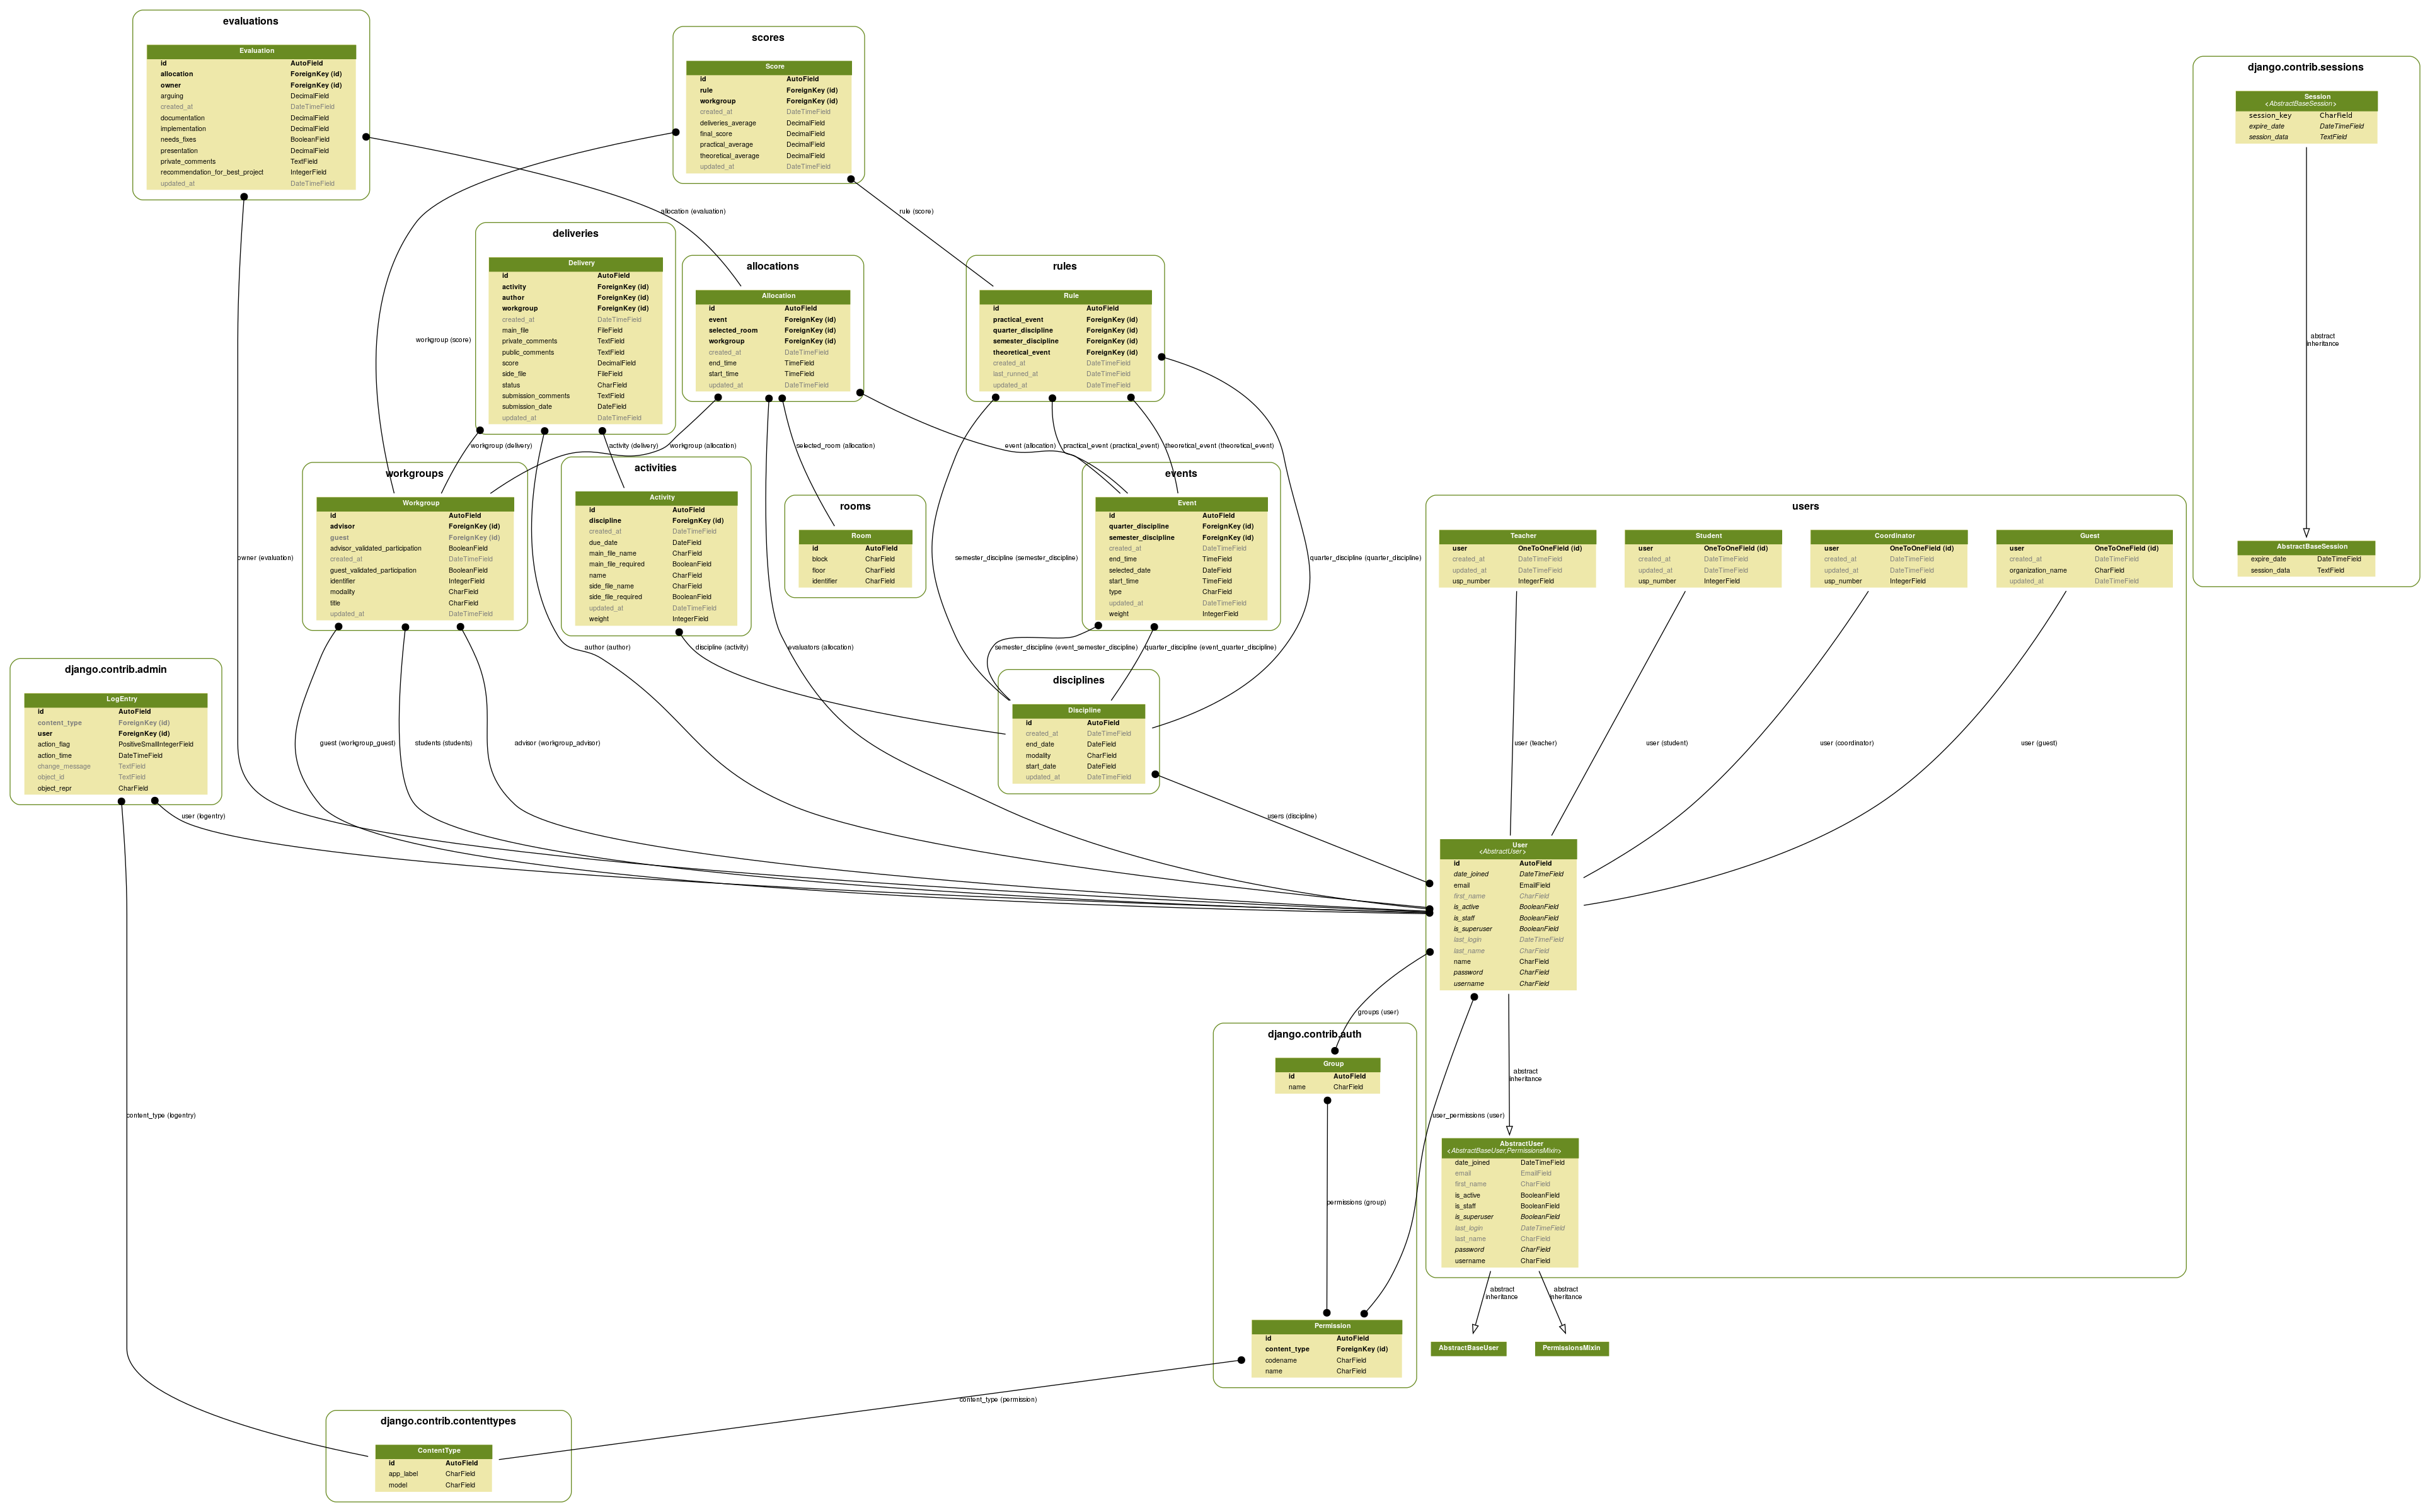
\includegraphics[angle=90, origin=c, scale=0.3]{imagens/output.png}
    \caption{Diagrama Entidade-Relacionamento do Sistema Desenvovlido, gerado automaticamente}
    \label{fig:output}
\end{figure}